\documentclass{article}
\usepackage{amssymb}
\usepackage{amsfonts}
\usepackage{tikz}
\usetikzlibrary{shapes, backgrounds}
\begin{document}
\title{1 Sentential Logic - Exercises}
\author{Scott Brown}
\maketitle
$\mathbb{N}$ is the set of natural numbers,\\
$\mathbb{Z}$ is the set of integers,\\
$\mathbb{Q}$ is the set of rational numbers and\\
$\mathbb{R}$ is the set of real numbers.\\

\subsection*{1.1 Deductive Reasoning and Logical Connectives}
1. (a) We'll have either a reading assignment or homework problems, but we
won't have both homework problems and a test.\\
$(R \vee H) \wedge \neg(H \wedge T)$\\
(b) You won't go skiing, or you will and there won't be any snow.\\
$\neg Ski \vee (Ski \wedge \neg Snow)$\\
(c) $\sqrt 7 \not \le 2$\\
$\neg (\sqrt 7 = 2) \wedge \neg (\sqrt 7 < 2)$\\
\linebreak
5. Let P = ``I will buy the pants''\\
   Let S = ``I will buy the shirt''\\
(a)$\neg(P \wedge \neg S)$\\
I will not buy the pants or I will buy the shirt.\\
(b)$\neg P \wedge \neg S$\\
I will not buy the pants and I will not buy the shirt.\\
(c)$\neg P \vee \neg S$\\
I will not buy the pants or I will not buy the shirt.\\
\subsection*{1.2 Truth Tables}
1.(a)
\linebreak
\begin{tabular}{cccc}
$\neg$&P&$\vee$&Q\\
\hline
F&T&\textbf{T}&T\\
F&T&\textbf{F}&F\\
T&F&\textbf{T}&T\\
T&F&\textbf{T}&F\\
\end{tabular}
\vspace{2em}
\linebreak
(b)
\linebreak
\begin{tabular}{ccccccccccccc}
(&S&$\vee$&G&)&$\wedge$&(&$\neg$&S&$\vee$&$\neg$&G&)\\
\hline
&T&T&T&&\textbf{F}&&F&T&F&F&T&\\
&T&T&F&&\textbf{T}&&F&T&T&T&F&\\
&F&T&T&&\textbf{T}&&T&F&T&F&T&\\
&F&F&F&&\textbf{F}&&T&F&T&T&F&\\
\end{tabular}
\vspace{2em}
\linebreak
2.(a)
\linebreak
\begin{tabular}{ccccccccccc}
$\neg$&[&P&$\wedge$&(&Q&$\vee$&$\neg$&P&)&]\\
\hline
\textbf{F}&&T&T&&T&T&F&T&&\\
\textbf{T}&&T&F&&F&F&F&T&&\\
\textbf{T}&&F&F&&T&T&T&F&&\\
\textbf{T}&&F&F&&F&T&T&F&&\\
\end{tabular}
\vspace{2em}
\linebreak
(b)
\linebreak
\begin{tabular}{cccccccccccc}
(&P&$\vee$&Q&)&$\wedge$&(&$\neg$&P&$\vee$&R&)\\
\hline
&T&T&T&&\textbf{T}&&F&T&T&T&\\
&T&T&F&&\textbf{T}&&F&T&T&T&\\
&F&T&T&&\textbf{T}&&T&F&T&T&\\
&F&F&F&&\textbf{F}&&T&F&T&T&\\
&T&T&T&&\textbf{F}&&F&T&F&F&\\
&T&T&F&&\textbf{F}&&F&T&F&F&\\
&F&T&T&&\textbf{T}&&T&F&T&F&\\
&F&F&F&&\textbf{F}&&T&F&T&F&\\
\end{tabular}
\vspace{2em}
\linebreak
3. The + symbol means \textit{exclusive or}\\
(a)
\linebreak
\begin{tabular}{ccc}
P&+&Q\\
\hline
T&\textbf{F}&T\\
T&\textbf{T}&F\\
F&\textbf{T}&T\\
F&\textbf{F}&F\\
\end{tabular}
\vspace{2em}
\linebreak
(b)
\begin{tabular}{cccccccccccc}
(&P&$\vee$&Q&)&$\wedge$&$\neg$&(&P&$\wedge$&Q&)\\
\hline
&T&T&T&&\textbf{F}&F&&T&T&T&\\
&T&T&F&&\textbf{T}&T&&T&F&F&\\
&F&T&T&&\textbf{T}&T&&F&F&T&\\
&F&F&F&&\textbf{F}&T&&F&F&F&\\
\end{tabular}
\vspace{2em}
\linebreak
4. Find a formula that is equivalent to $P \vee Q$\\
\begin{tabular}{cccccccc}
$\neg$&(&$\neg$&P&$\wedge$&$\neg$&Q&)\\
\hline
\textbf{T}&&F&T&F&F&T&\\
\textbf{T}&&F&T&F&T&F&\\
\textbf{T}&&T&F&F&F&T&\\
\textbf{F}&&T&F&T&T&F&\\
\end{tabular}
\vspace{2em}
\linebreak
5. Some mathematicians use the symbol $\downarrow$ to mean \textit{nor}\\
(a)Make a truth table for $P \downarrow Q$\\
\begin{tabular}{ccc}
P&$\downarrow$&Q\\
\hline
T&\textbf{F}&T\\
T&\textbf{F}&F\\
F&\textbf{F}&T\\
F&\textbf{T}&F\\
\end{tabular}
\vspace{2em}
\linebreak
(b) Find a formula using only the connectives $\wedge$,$\vee$ and $\neg$ that is equivalent to $P \downarrow Q$.\\
\begin{tabular}{ccccc}
$\neg$&P&$\wedge$&$\neg$&Q\\
\hline
F&T&\textbf{F}&F&T\\
F&T&\textbf{F}&T&F\\
T&F&\textbf{F}&F&T\\
T&F&\textbf{T}&T&F\\
\end{tabular}
\vspace{2em}
\linebreak
(c) Find formulas using only the connective $\downarrow$ that are equivalent to $\neg P$, $P \vee Q$ and $P \wedge Q$.\\
$\neg P$:\\
\begin{tabular}{ccc}
P&$\downarrow$&P\\
\hline
T&\textbf{F}&T\\
F&\textbf{T}&F\\
\end{tabular}
\vspace{2em}
\linebreak
$P \vee Q$:\\
\begin{tabular}{ccccccccccc}
(&P&$\downarrow$&Q&)&$\downarrow$&(&P&$\downarrow$&Q&)\\
\hline
&T&F&T&&\textbf{T}&&T&F&T&\\
&T&F&F&&\textbf{T}&&T&F&F&\\
&F&F&T&&\textbf{T}&&F&F&T&\\
&F&T&F&&\textbf{F}&&F&T&F&\\
\end{tabular}
\vspace{2em}
\linebreak
6. $P | Q$ means \textit{nand}, "P and Q are not both true".\\
(a) Truth table for $P | Q$\\
\begin{tabular}{ccc}
$P$&$|$&$Q$\\
\hline
T&\textbf{F}&T\\
T&\textbf{T}&F\\
F&\textbf{T}&T\\
F&\textbf{T}&F\\
\end{tabular}
\vspace{2em}
\linebreak
(b)\begin{tabular}{cccccc}
$\neg$&(&$P$&$\wedge$&$Q$&)\\
\hline
\textbf{F}&&T&T&T&\\
\textbf{T}&&T&F&F&\\
\textbf{T}&&F&F&T&\\
\textbf{T}&&F&F&F&\\
\end{tabular}
\vspace{2em}
\linebreak
(c) Equivalent to $\neg P$ using $|$\\
\begin{tabular}{ccc}
$P$&$|$&$P$\\
\hline
T&\textbf{F}&T\\
F&\textbf{T}&F\\
\end{tabular}
\vspace{2em}
\linebreak
7. Use truth tables to determine whether or not these arguments are valid.\\
(a)\\
Let $Jm$ = "Jane wins the maths prize"\\
Let Pm = "Pete wins the maths prize"\\
Let Pc = "Pete wins the chemistry prize"\\

\begin{tabular}{ccc}
$Jm$&$|$&Pm\\
Pm&$\vee$&Pc\\
$Jm$&&\\
\hline
$\therefore$ Pc
\end{tabular}
\vspace{2em}
\linebreak
\begin{tabular}{c|c|c|c|c}
$Pm$&$Pc$&$Jm$&$Jm | Pm$&$Pm \vee Pc$\\
\hline
T&T&T&F&T\\
T&F&T&F&T\\
F&T&T&T&T\\
F&F&T&T&F\\
T&T&F&T&T\\
T&F&F&T&T\\
F&T&F&T&T\\
F&F&T&T&F\\
\end{tabular}
\vspace{2em}
\linebreak
When the premises are all true, the conclusion is true, so the argument is valid.\\
\linebreak
(b) Let B = "beef"\\
 Let F = "fish"\\
 Let P = "peas"\\
 Let C = "corn"\\
 \begin{tabular}{ccc}
 $B + F$\\
 $P + C$\\
 $F | C$\\
 \hline
 $\therefore B | P$\\
 \end{tabular}
 \vspace{2em}
 \linebreak
 \begin{tabular}{cccccccc}
 B&F&P&C&$B + F$&$P + C$&$F | C$&$B | P$\\
 \hline
 T&T&T&T&F&F&F&F\\
 T&F&T&T&T&F&T&F\\
 F&T&T&T&T&F&F&T\\
 F&F&T&T&F&F&T&T\\
 T&T&F&T&F&T&F&T\\
 T&F&F&T&T&T&T&T\\
 F&T&F&T&T&T&F&T\\
 F&F&F&T&F&T&T&T\\
 T&T&T&F&F&T&T&F\\
 T&F&T&F&T&T&T&F\\
 F&T&T&F&T&T&T&T\\
 F&F&T&F&F&T&T&T\\
 T&T&F&F&F&F&T&T\\
 T&F&F&F&T&F&T&T\\
 F&T&F&F&T&F&T&T\\
 F&F&F&F&F&F&T&T\\
 \end{tabular}
 \vspace{2em}
 \linebreak
 The argument is invalid because the conclusion can be wrong even when all of the premises are true.\\
 \linebreak
 (c) Let J = "John is telling the truth"\\
         S = "Sam is telling the truth"\\
         B = "Bill is telling the truth"\\
         
  \begin{tabular}{cc}
  $J \vee B$& "Either John or Bill is telling the truth"\\
  $S | B$  &  "Either Sam or Bill is lying"\\
  \hline
  $\therefore J \vee \neg S$& "Therefore either John is telling the truth or Sam is lying"\\
  \end{tabular}         
  \vspace{2em}
 \linebreak
 \begin{tabular}{cccccc}
 J&B&S&$J \vee B$&$S | B$&$J \vee \neg S$\\
  \hline
 T&T&T&T&F&T\\
 T&F&T&T&T&T\\
 F&T&T&T&F&F\\
 F&F&T&F&T&F\\
 T&T&F&T&T&T\\
 T&F&F&T&T&T\\
 F&T&F&T&T&T\\
 F&F&F&F&T&T\\
 \end{tabular}
   \vspace{2em}
 \linebreak
 The argument is valid because when the premises are true, the conclusion is always true.\\
 \linebreak
 (d)Let S = "Sales will go up"\\
 Let E = "Expenses will go up"\\
 Let B = "The boss will be happy"\\
 \begin{tabular}{c}
 $(S \wedge B) \vee (E \wedge \neg B)$\\
 \hline
 $\therefore S | E$\\
 \end{tabular}
  \vspace{2em}
 \linebreak
 \begin{tabular}{c|c|c|c|c|c|c}
 S&E&B&$S \wedge B$&$E \wedge \neg B$&$(S \wedge B) \vee (E \wedge \neg B)$&$S | E$\\
 \hline
 T&T&T&T&F&T&F\\
 T&F&T&T&F&T&T\\
 F&T&T&F&F&F&T\\
 F&F&T&F&F&F&T\\
 T&T&F&F&T&T&F\\
 T&F&F&F&F&F&T\\
 F&T&F&F&T&T&T\\
 F&F&F&F&F&F&T\\
 \end{tabular}
  \vspace{2em}
 \linebreak
 The argument is invalid because the conclusion can be false even when the premise is true.\\
 \newline
 
9. Use truth tables to determine which of these statements are tautologies, which are contradictions, and which are neither.\\
\newline
(a)$(P \vee Q)\wedge (\neg P \vee \neg Q)$ is neither a tautology nor a contradiction\\
\begin{tabular}{c|c|c|c|c|c|c}
$P$&$Q$&$\neg P$&$\neg Q$&$P \vee Q$&$\neg P \vee \neg Q$&$(P \vee Q)\wedge (\neg P \vee \neg Q)$\\
\hline
T&T&F&F&T&F&F\\
T&F&F&T&T&T&T\\
F&T&T&F&T&T&T\\
F&F&T&T&F&T&F\\
\end{tabular} 
\vspace{2em}
 \linebreak
 
 (b) $(P \vee Q)\wedge (\neg P \wedge \neg Q)$ is a contradiction\\
 \begin{tabular}{c|c|c|c|c|c|c}
 $P$&$Q$&$\neg P$&$\neg Q$&$P \vee Q$&$\neg P \wedge \neg Q$&$(P \vee Q)\wedge (\neg P \wedge \neg Q)$\\
 \hline
 T&T&F&F&T&F&F\\
 T&F&F&T&T&F&F\\
 F&T&T&F&T&F&F\\
 F&F&T&T&F&T&F\\
 \end{tabular}
 \vspace{2em}
 \linebreak
 
 (c)$(P \vee Q)\vee (\neg P \vee \neg Q)$ is a tautology\\
 \begin{tabular}{c|c|c|c|c|c|c}
 $P$&$Q$&$\neg P$&$\neg Q$&$P \vee Q$&$\neg P \vee \neg Q$&$(P \vee Q)\vee (\neg P \vee \neg Q)$\\
 \hline
 T&T&F&F&T&F&T\\
 T&F&F&T&T&T&T\\
 F&T&T&F&T&T&T\\
 F&F&T&T&F&T&T\\
 \end{tabular}
 \vspace{2em}
 \linebreak
 (d)$[P \wedge (Q \vee \neg R)]\vee (\neg P \vee R)$ is a tautology\\
 \begin{tabular}{ccccccccccc}
 $[P$&$\wedge$&$(Q$&$\vee$&$\neg$&$R)]$&$\vee$&$(\neg$&$P$&$\vee$&$R)$\\
 \hline
 T&T&T&T&F&T&\textbf{T}&F&T&T&T\\
 T&F&F&F&F&T&\textbf{T}&F&T&T&T\\
 F&F&T&T&F&T&\textbf{T}&T&F&T&T\\
 F&F&F&F&F&T&\textbf{T}&T&F&T&T\\
 T&T&T&T&T&F&\textbf{T}&F&T&F&F\\
 T&T&F&T&T&F&\textbf{T}&F&T&F&F\\
 F&F&T&T&T&F&\textbf{T}&T&F&T&F\\
 F&F&F&T&T&F&\textbf{T}&T&F&T&F\\
 \end{tabular}
 \vspace{2em}
 \linebreak
 \newline
11. (a) $\neg(\neg P \wedge \neg Q) \equiv P \vee Q$\\
(b)$(P \wedge Q) \vee (P \wedge \neg Q) \equiv P$\\
(c) $\neg(P \wedge \neg Q) \vee (\neg P \wedge Q) \equiv (\neg P \vee Q) \vee (\neg P \wedge Q)$\\
 
 
 15. A statement with $n$ letters requires $2^n$ rows\\
 
 16.\\
 \begin{tabular}{c|c|c}
 P&Q&$P \vee \neg Q$\\
 \hline
 F&F&T\\
 F&T&F\\
 T&F&T\\
 T&T&T\\
 \end{tabular}
  \vspace{2em}
 \linebreak
 
 \subsection*{1.3. Variables and Sets}
 1.(a) 3 is a common divisor of 6, 9 and 15.\\
 $3 | x \wedge x \in \{6,9,15 \}$\\
 (b) x is divisible by both 2 and 3 but not 4.\\
 $(2 | x) \wedge (3 | x) \wedge \neg (4 | x)$\\
 (c)x and y are natural numbers, and exactly one of them is prime.\\
 $x, y \in \mathbb{N} \wedge (prime(x) \vee prime(y)) \wedge \neg (prime(x) \wedge prime(y)) $\\
 3. Write definitions using elementhood tests for the following sets.\\
 (a) \{Mercury, Venus, Earth, Mars, Jupiter, Saturn, Uranus, Neptune, Pluto\}\\
 \{x $|$ x is a planet of this solar system\}\\
 (b)\{Brown, Columbia, Cornell, Dartmouth, Harvard, Princeton, University of Pennsylvania, Yale\}\\
 \{x $|$ x is an American university\}\\
 (c) \{Alabama, Alaska, Arizona,...,Wisconsin, Wyoming\}\\
 \{x $|$ x is an American state\}\\
 (d) \{Alberta, British Columbia,...,Yukon\}\\
 \{x $|$ x is a Canadian province\}\\
4.(a) \{1,4,9,16,25,36,49,64,...\}\\
\{x $|$ x = $n^2 \wedge n \in \mathbb{N}$\}\\
(b)\{1,2,4,8,16,32,64,...\}\\
\{n $| n \in \mathbb{N} \wedge n = (n-1)*2$\}\\
5.(a) $-3 \in \{x \in \mathbb{R} | 13 - 2x > 1\}$.\\
$x$ is bound and there are no free variables. 13 - (2 * -3)=13 + 6 = 19. 19 $>$ 1 so the statement is true.\\
(b)$4 \in \{x \in \mathbb{R^-} | 13 - 2x > 1 \}$\\
$x$ is bound and there are no free variables. 4 is not a member of the set of negative real numbers, so the statement is false.\\
(c) $5 \not \in \{x \in \mathbb{R} | 13 -2x > c\}$\\
$x$ is bound and $c$ is free.\\
7. Truth sets\\
(c) x is the author of this book. = \{ Daniel J. Velleman \}\\
8. Truth sets\\
(a) $x \in \mathbb{R} \wedge x^2 -4x + 3 = 0$\\
$(x -3)(x - 1) = 0$\\
$\{x | x \in \mathbb{R} \wedge x^2 - 4x + 3 = 0\} = \{1,3\}$\\
(b)$x \in \mathbb{R} \wedge x^2 -2x + 3 = 0$\\
= $\{ (1 + \sqrt 2i)(1 - \sqrt 2i)\}$\\
(c)$x \in \mathbb{R} \in 5 \wedge \{y \in \mathbb{R} | x^2 + y^2 < 50\}$\\
$\{x | x \in \mathbb{R} \in 5 \wedge \{y \in \mathbb{R} | x^2 + y^2 < 50\}\} = \{1,2,3,4\}$\\
\subsection*{1.4 Operations on Sets}
1. Let $A = \{1,3,12,35\}$, $B = \{3,7,12,20\}$,$C = \{x | x$ is a prime number \}\\
(a)$A \cap B = \{3,12\}$\\
(b)$(A \cup B) \setminus C = \{1,12,20,35\}$.\\
(c)$(A \cup (B \setminus C) = \{1,3,12,20,35\}$\\
\newline
4. Use Venn diagrams to verify the following identities:\\
(a) $A \ (A \cap B) = A \setminus B$.\\

\begin{center}
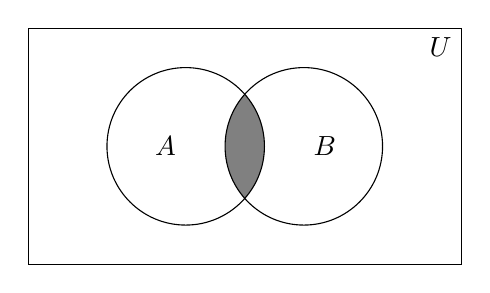
\begin{tikzpicture}
\draw (-2,-1.5) rectangle (3.5,1.5) node[below left]{$U$
};
\begin{scope} % start of clip scope
\clip (0,0) circle (1cm);
\fill[gray] (1.5,0) circle (1cm);
\end{scope} % end of clip scope
\draw (0,0) circle (1cm) node[left] {$A$};
\draw (1.5,0) circle (1cm) node[right] {$B$};
\end{tikzpicture}
\end{center}
(b) $A \cup (B \cap C) = (A \cup B) \cap (A \cup C)$\\
\newline
8.(a)$(A \setminus B) \setminus C \equiv A \wedge \neg(B \vee C) $\\
(b)$A \setminus (B \setminus C)\equiv A \wedge \neg(B \wedge \neg C)$\\
(c)$(A \setminus B) \cup (A \cap C)\equiv (A \wedge \neg B) \vee (A \wedge C)$\\
(d)$(A \setminus B) \cap (A \setminus C) \equiv (A \wedge \neg B)\wedge (A \wedge \neg C)$\\
(e)$A \setminus (B \cap C) \equiv A \wedge \neg (B \wedge C)$\\
\newline
\subsection*{1.5. The Conditional and Biconditional Connectives}
1. Analyse the logical forms of these statements:
(a) If this gas either has an unpleasant smell or is not explosive, then it isn't hydrogen.\\
$(S \vee \neg E)\Rightarrow \neg H$\\
(b) Having both a fever and a headache is a sufficient condition for George to go to the doctor.\\
$(F \wedge H)\Rightarrow D$\\
(c) Both having a fever and having a headache are sufficient conditions for George to go to the doctor.\\
$(F \vee H) \Rightarrow D$\\
(d) If $x \not = 2$, then a necessary condition for $x$ to be prime is that $x$ be odd.\\
$x \not = 2 \Rightarrow Prime(x) \Rightarrow Odd(x)$\\
\newline
4.(a)Let S = "Sales will go up"\\
 Let E = "Expenses will go up"\\
 Let B = "The boss will be happy"\\
 \begin{tabular}{c}
 $(S \wedge B) \vee (E \wedge \neg B)$\\
 \hline
 $\therefore S | E$\\
 \end{tabular}
  \vspace{2em}
 \linebreak
 \begin{tabular}{c|c|c|c|c|c|c}
 S&E&B&$S \wedge B$&$E \wedge \neg B$&$(S \wedge B) \vee (E \wedge \neg B)$&$S | E$\\
 \hline
 T&T&T&T&F&T&F\\
 T&F&T&T&F&T&T\\
 F&T&T&F&F&F&T\\
 F&F&T&F&F&F&T\\
 T&T&F&F&T&T&F\\
 T&F&F&F&F&F&T\\
 F&T&F&F&T&T&T\\
 F&F&F&F&F&F&T\\
 \end{tabular}
  \vspace{2em}
 \linebreak
 The argument is invalid because the conclusion can be false even when the premise is true.\\
 \newline
 (b) 
 \begin{tabular}{cc}
 $(T \wedge U)\Rightarrow R$&"If the tax rate and unemployment both go up,then there will be a recession"\\
 $G \Rightarrow \neg R$&"If the GNP goes up, then there will not be a recession"\\
 $G \wedge T$&"The  GNP and taxes are both going up"\\
 \hline
 $\therefore \neg U$&"Therefore the unemployment rate is not going up"\\
 \end{tabular}
 \vspace{2em}
 \linebreak
 \begin{tabular}{cccccccccccccc}
 ($T$&$\wedge$&$U$)&$\Rightarrow$&$R$&$G$&$\Rightarrow$&$\neg$&$R$&$G$&$\wedge$&$T$&$\neg$&$U$\\
 \hline
 T&T&T&T&T&T&F&F&T&T&T&T&\textbf{F}&T\\
 T&F&F&T&T&T&F&F&T&T&T&T&\textbf{T}&F\\
 F&F&T&T&T&T&F&F&T&T&F&F&\textbf{F}&T\\
 F&F&F&T&T&T&F&F&T&T&F&F&\textbf{T}&F\\
 T&T&T&F&F&T&T&T&F&T&T&T&\textbf{F}&T\\
 T&F&F&T&F&T&T&T&F&T&T&T&\textbf{T}&F\\
 F&F&T&T&F&T&T&T&F&T&F&F&\textbf{F}&T\\
 F&F&F&T&F&T&T&T&F&T&F&F&\textbf{T}&F\\
 T&T&T&T&T&F&T&F&T&F&F&T&\textbf{F}&T\\
 T&F&F&T&T&F&T&F&T&F&F&T&\textbf{T}&F\\
 F&F&T&T&T&F&T&F&T&F&F&F&\textbf{F}&T\\
 F&F&F&T&T&F&T&F&T&F&F&F&\textbf{T}&F\\
 T&T&T&F&F&F&T&T&F&F&F&T&\textbf{F}&T\\
 T&F&F&T&F&F&T&T&F&F&F&T&\textbf{T}&F\\
 F&F&T&T&F&F&T&T&F&F&F&F&\textbf{F}&T\\
 F&F&F&T&F&F&T&T&F&F&F&F&\textbf{T}&F\\
 \end{tabular}
  \vspace{2em}
  \linebreak
  The argument is valid because when all of the premises are true, the conclusion is also true.\\
  \newline
  (c)\begin{tabular}{cc}
  $L \Leftrightarrow (H \wedge C)$&"Warning light if and only if the pressure is too high and the relief valve is clogged"\\
  $\neg C$&"The relief valve is not clogged"\\
  \hline
  $\therefore L \Leftrightarrow H$&"Therefore warning light if and only if pressure is too high"\\
  \end{tabular}
 \vspace{2em}
 \linebreak
 \begin{tabular}{c|c|c|c|c|c|c}
 L&H&C&$H \wedge C$&$L \Leftrightarrow (H \wedge C)$&$\neg C$&$\therefore L \Leftrightarrow H$\\
 \hline
 T&T&T&T&T&F&T\\
 T&F&T&F&F&F&F\\
 F&T&T&T&F&F&F\\
 F&F&T&F&T&F&T\\
 T&T&F&F&F&T&T\\
 T&F&F&F&F&T&F\\
 F&T&F&F&T&T&F\\
 F&F&F&F&T&T&T\\
 \end{tabular}
 \vspace{2em}
 \linebreak
 The argument is invalid because the conclusion can be false even when the premises are true.\\
\end{document}